\documentclass[12pt,a4paper,openany,ngerman,plainfootsepline,plainheadsepline]{scrbook}
% Change "article" to "report" to get rid of page number on title page
\usepackage{amsmath,amsfonts,amsthm,amssymb}
\usepackage{setspace}
\usepackage{Tabbing}
\usepackage{lastpage}
\usepackage[backend=biber,citestyle=verbose-note]{biblatex}
\addbibresource{bib/verzeichnis1.bib}
\usepackage{here} 
\usepackage{tocbasic}
\usepackage{color}
\usepackage{listings}
\usepackage{pifont}


\usepackage[automark,						%Automatische Kopfzeile
						%headtopline,				%Linie �ber dem Seitenkopf
						%plainheadtopline,	%Plain, Linie �ber dem Seitenkopf
						headsepline,				%Linie zwischen Kopf und Textk�rper
						%plainheadsepline,	%Plain, Linie zwischen Kopf und Textk�rper
						footsepline,				%Linie zwischen Textk�rper und Fu�
						plainfootsepline,   %Plain, Linie zwischen Textk�rper und Fu�
						%footbotline,				%Linie unter dem Fu�
						%plainfootbotline   %Plain, Linie unter dem Fu�
						]{scrpage2}
\usepackage{graphicx,wrapfig}
\usepackage[ansinew]{inputenc}
\usepackage[ngerman]{babel}

\usepackage[hidelinks]{hyperref}


% In case you need to adjust margins:
\topmargin=-0.45in      %
\evensidemargin=0in     %
\oddsidemargin=0in      %
\textwidth=6.5in        %
\textheight=9.0in       %
\headsep=0.25in         %
\setcounter{secnumdepth}{3}
\setcounter{tocdepth}{3}
%\pdfliteral direct {/Interpolate true}
%\special {pdf:direct: /Interpolate true }
% Homework Specific Information
\newcommand{\hmwkTitle}{Racketsports Manager}
\newcommand{\hmwkClass}{Semesterarbeit ZHAW}
\newcommand{\hmwkAuthorName}{Raphael Marques}
\newcommand{\hmwkTeacherName}{Michael Reiser}


                                   %
\clearscrplain		
%Alte Plain-Formatierung entfernen
\cehead{\headmark}    % Chaper auf geraden Seiten (links) in Kopfzeile
\cohead{\headmark}
\rehead{
\includegraphics[width=25pt]{Graphics/zhaw.jpg}}    % Section auf ungeraden Seiten (rechts) in Kopfzeile
\rohead{
\includegraphics[width=25pt]{Graphics/zhaw.jpg}} 
\lehead{\hmwkTitle}    % Section auf ungeraden Seiten (rechts) in Kopfzeile
\lohead{\hmwkTitle} 
\refoot{\hmwkAuthorName}    % Chaper auf geraden Seiten (links) in Kopfzeile
\rofoot{\hmwkAuthorName}
\lofoot{Page\ \thepage\ of\ \pageref{LastPage}}    % Chaper auf geraden Seiten (links) in Kopfzeile
\lefoot{Page\ \thepage\ of\ \pageref{LastPage}}
\setheadsepline{0.4pt}   
\setfootsepline{0.4pt}                                  %
\pagestyle{scrheadings}
\automark[section]{chapter}
 % Seitenstil aktivieren
\renewcommand{\chapterpagestyle}{scrheadings}
% This is used to trace down (pin point) problems
% in latexing a document:
%\tracingall
\pdfpxdimen=1in

\divide\pdfpxdimen by 800

%%%%%%%%%%%%%%%%%%%%%%%%%%%%%%%%%%%%%%%%%%%%%%%%%%%%%%%%%%%%%
% Make title
\title{\vspace{1in}\textmd{\textbf{\ \hmwkTitle}}
\\\normalsize \vspace{0.1in} \large{\hmwkClass} \vspace{0.5in}
\\
\includegraphics[width=300pt]{Graphics/title.png}
\vspace{0.1in}\large{\textit{}}\vspace{0.2in}
\author{\textbf{Autor: \hmwkAuthorName}
\\\textbf{ Betreuer: \hmwkTeacherName}}}
%%%%%%%%%%%%%%%%%%%%%%%%%%%%%%%%%%%%%%%%%%%%%%%%%%%%%%%%%%%%%



\begin{document}
\nocite{*}
\begin{spacing}{1.1}

\maketitle
\newpage
% Uncomment the \tableofcontents and \newpage lines to get a Contents page
% Uncomment the \setcounter line as well if you do NOT want subsections
%       listed in Contents
%\setcounter{tocdepth}{1}
%\tableofcontents
%\newpage

% When problems are long, it may be desirable to put a \newpage or a
% \clearpage before each homeworkProblem envirosnment

\clearpage
\begin{normalsize}
\setcounter{tocdepth}{2}
\tableofcontents
% !TeX spellcheck = de_CH


\chapter{Inhalt der Arbeit}

\section{Motivation}


\section{Aufgabenstellung}


\section{Vorgehen}


\section{Zielsetzung der Arbeit}

% !TeX spellcheck = de_CH
% !TeX spellcheck = de_CH
% !TeX spellcheck = de_CH
% !TeX spellcheck = de_CH
\chapter{Implementation}

\section{Projektaufbau}
Um den Projektaufbau zu erkl�ren wird zuerst die Ordnerstruktur angeschaut:
\begin{figure}[ht]
	\centering
	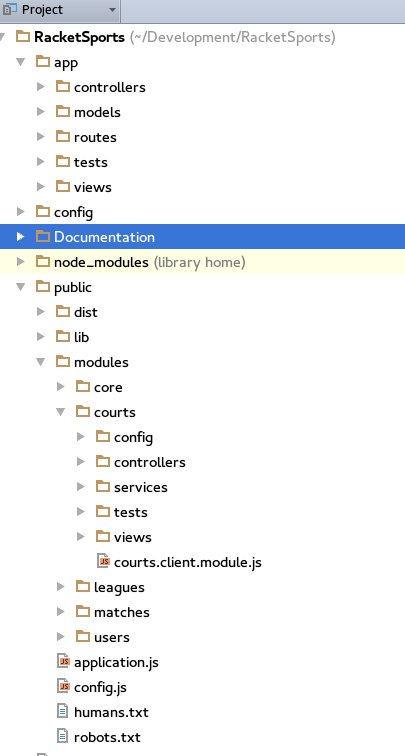
\includegraphics[width=0.3\textwidth]{Graphics/projectsetup.png}
	\caption{Projekt Ordner Struktur}
	\label{ProjectSetup}
	\end{figure}
Wie auf der Graphik ersichtlich besteht das Projekt aus den �berordnern App, Documentation und public. Node\textunderscore modules ist ein System-Ordner und muss hier nicht betrachtet werden.
\subsection{app}


\begin{itemize}
	\itemsep-0.4em
	\item Controller - Kontroller im MVC
	\item Models - Definition der Datenobjekte
	\item Routers - Routing definition durch das MVC
	\item Tests - Unittests f�r Controller und Models
	\item Views - Verschiedene Basisviews, welche noch nicht zum Client gesendet wurden
\end{itemize}

\subsection{Documentation}
Der Ordner Documentation beinhaltet diese Dokumentation sowie alle Pr�sentationen.

\subsection{public}
Public beinhaltet alle Files, welche an den Client gesendet werden.
\begin{itemize}
	\itemsep-0.4em
	\item dist - Beinhaltet definitionen, welche Ordner gesendet werden, was f�r Module wo registriert werden sollen
	\item lib - binhaltet statische Libraries, welche der Client braucht. Hier befinden sich nodeJS, AngularJS und Bootstrap als libraries.
	\item modules - Hier ist die Eigentliche Client Logik versteckt. F�r jedes Modul gibt es folgende Ordner:
	\begin{itemize}
	\itemsep -0.4 em
		\item config - Konfiguration von Modul und Client Routing. Definiert z.b. was f�r Items �ber den Header ansprechbar sind
		\item controller - AngularJS Controller
		\item services - Definiert den Link zur API
		\item tests - Unit Tests f�r die AngularJS Module
		\item views - Definiert views f�r die einzelnen Seiten der Applikation.
	\end{itemize}

\end{itemize}

\section{REST API}
Die REST API besteht aus f�nf Endpunkten:
\begin{itemize}
	\itemsep-0.8em
	\item /matches - Stellt alle Operationen f�r Matches zur Verf�gung
	\item /leagues - Stellt alle Operationen f�r Liga Management zur Verf�gung
	\item /courts - Stellt alle Operationen f�r die Verwaltung von Racketsportzentren zur Verf�gung
	\item /users - Stellt alle Operationen f�r das Usermanagemnt zur Verf�gung
	\item /core - Stellt Core-Funktionalit�ten (Home Seite) zur Verf�gung
\end{itemize}
Die Endpunkte /users und /core waren im MEANJS Stack schon vorhanden. Der User Endpunkt wurde jedoch modifiziert. Die Modifizierungen sind in dem Kapitel dokumentiert, die schon vorhandenen Endpunkte nicht. 

\subsection{Routing}
Um die REST API anzusteuern gibt es ein zentrales Routing in der Applikation. Dieses Routing definiert, welche URL welche Funktion aufruft. Jedes Modul hat eine eigene Routing Definition um das die einzelnen Files �bersichtlich zu halten. 

Folgendes Codebeispiel zeigt das Routing des Courts Moduls. Es definiert URLs und HTTP Methoden wie die URL aufgerufen wird. Je nach Methode werden anschliessend verschiedene Parameter definiert, zum Beispiel wie der Endpunkt gesch�tzt ist (requires Login, hat Autorisierung) und anschliessend welche Funktion aufgerufen wird (courts.update)

\begin{lstlisting}
module.exports = function(app) {
var users = require('../../app/controllers/
		users.server.controller');
var courts = require('../../app/controllers/
		courts.server.controller');

// Courts Routes
app.route('/courts')
.get(courts.list)
.post(users.requiresLogin, courts.create);

app.route('/courts/:courtId')
.get(courts.read)
.put(users.requiresLogin, courts.hasAuthorization, courts.update)
.delete(users.requiresLogin, courts.hasAuthorization,
 courts.delete);
app.route('/courts/:courtId/join')
.get(users.requiresLogin, courts.join);
app.route('/courts/:courtId/leave')
.get(users.requiresLogin, courts.leave);
// Finish by binding the Court middleware
app.param('courtId', courts.courtByID);
};

\end{lstlisting}

Am Anfang (Linie 2 und 4) der Routen werden die Controller inkludiert, damit die Funktionen auch gefunden werden.


\subsection{Spiel Endpunkt /matches}
\begin{figure}[ht]
	\centering
	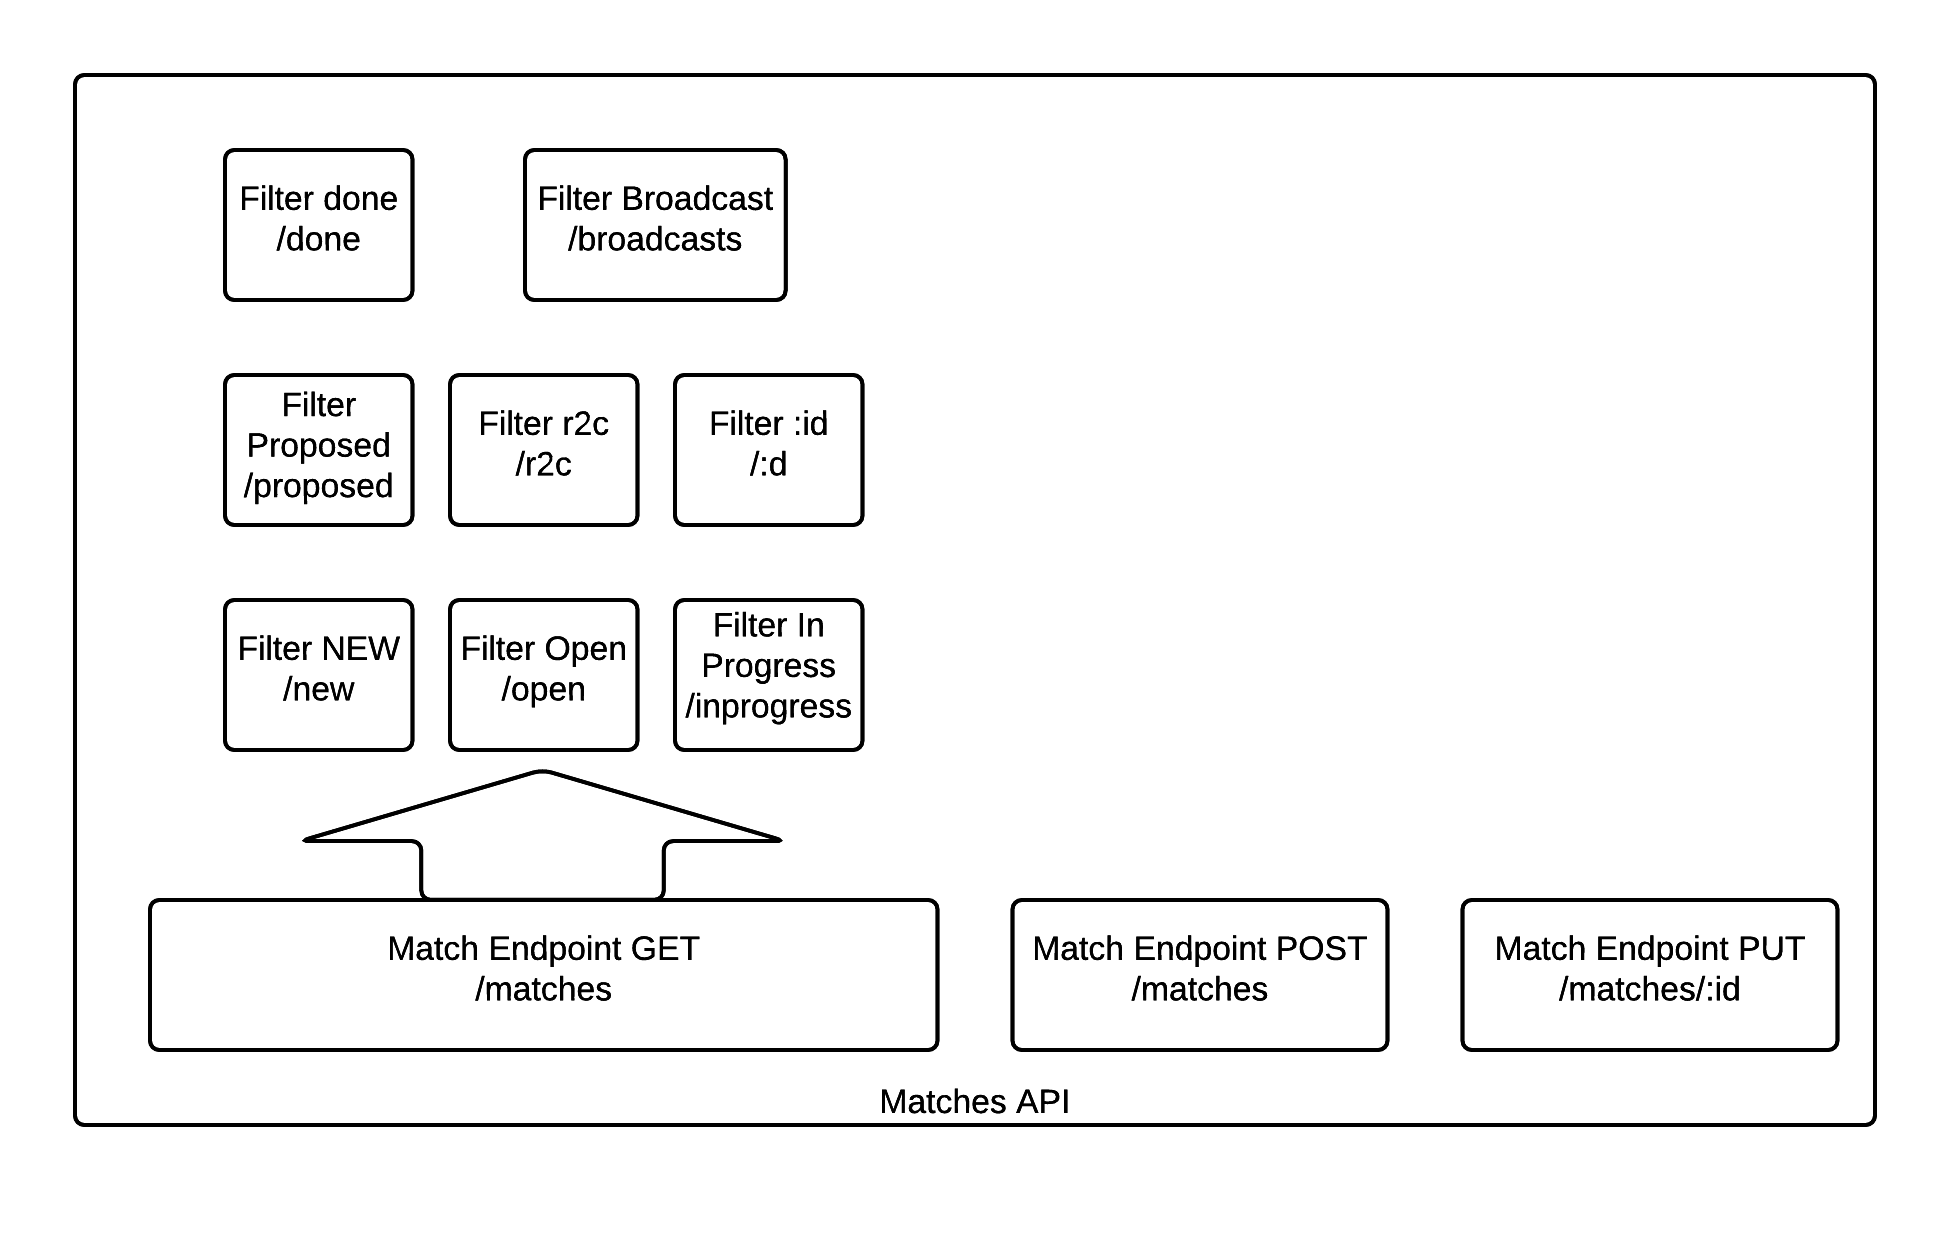
\includegraphics[width=0.8\textwidth]{Graphics/api_match.png}
	\caption{API f�r Spiele}
	\label{MatchAPI}
\end{figure}

Bei allen Match Endpunkten muss der User als Spieler registriert sein, um Informationen �ber das Spiel zu erhalten. Ausnahme ist, wenn er direkt die ID eingibt und direkt auf Spiel Detauls zugreift. 

Mit einem Post f�gt man der Datenbank ein Spiel hinzu, mit PUT aktualisiert man das Spiel mit neuen oder ge�nderten Daten. Hinter dem PUT interface gibt es gewisse Input Validations um Missbrauch zu verhindern. In dieser ersten Version sin ddie Validations jedoch relativ einfach gehalten. 

Um eine gute �bersicht aller Spiele auf der List Matches View zu erstelllen, gibt es f�r jeden Status eines Spieles einen eigenen API Call (/matches/new, /matches/open, /matches/inprogress, /matches/proposed, /matches/r2c, /matches/done). 

Der API Endpunkt /matches/broadcast listet zus�tzlich alle broadcasting Anfragen auf. Der Conntroller des Enpunkt Korreliert, in welchen Racketsportzentren der User registriert ist und die Matches ohne zweiten Spieler und gibt das Resultat dem Client.

\subsubsection{Codebeispiel - Filtering und Population von Unterobjekten}
Um bei den Spielen nur die offene Spiele zu finden, wird in der Datenbank auf den Status des Spiels gefiltert. Dies wird �ber einen Select auf die JSON Eigenschaft gemacht:
\begin{lstlisting}
exports.listOpen = function(req, res) {
	var user = req.user;
Match.find({'spieler.user': req.user, state: 'open'})
	.sort('-created').populate('spieler court')
	.exec(function(err, matches) {
		User.populate(matches, {path: 'spieler.user'},
		function (err, user) {
		if (err) {
			return res.status(400).send({
			message: errorHandler.getErrorMessage(err)
		});
		} else {
			res.jsonp(matches);
		}
		});
	});
};
\end{lstlisting}
Auf der Zeile 3 ist der Select f�r die Datenbank zu finden. Ein Teil des zu suchenden Objektes wird definiert als erster Parameter der Match.find() Methode.

Das Match Objekt beinhaltet Spieler sowie Courts. Diese Felder sind jedoch nur IDs auf andere Objekte (Als Beispiel: ObjectID(AA4335GE0DE9EV88A) ). Um auf Datenfehler der Unterobjekte zugreifen zu k�nnen, m�ssen die Objekte popularisiert werden. Auf der Zeile 4 erkennt man, dass f�r das Objekt Match die Unterobjekte Spieler sowie Courts popularisiert werden. Nun hat das Objekt Spieler zus�tzlich Unterobjekte. Hier muss man eine neue Population des Objektes User ausf�hren (siehe Zeile 6).



\subsection{Liga Endpunkt}

\begin{figure}[ht]
	\centering
	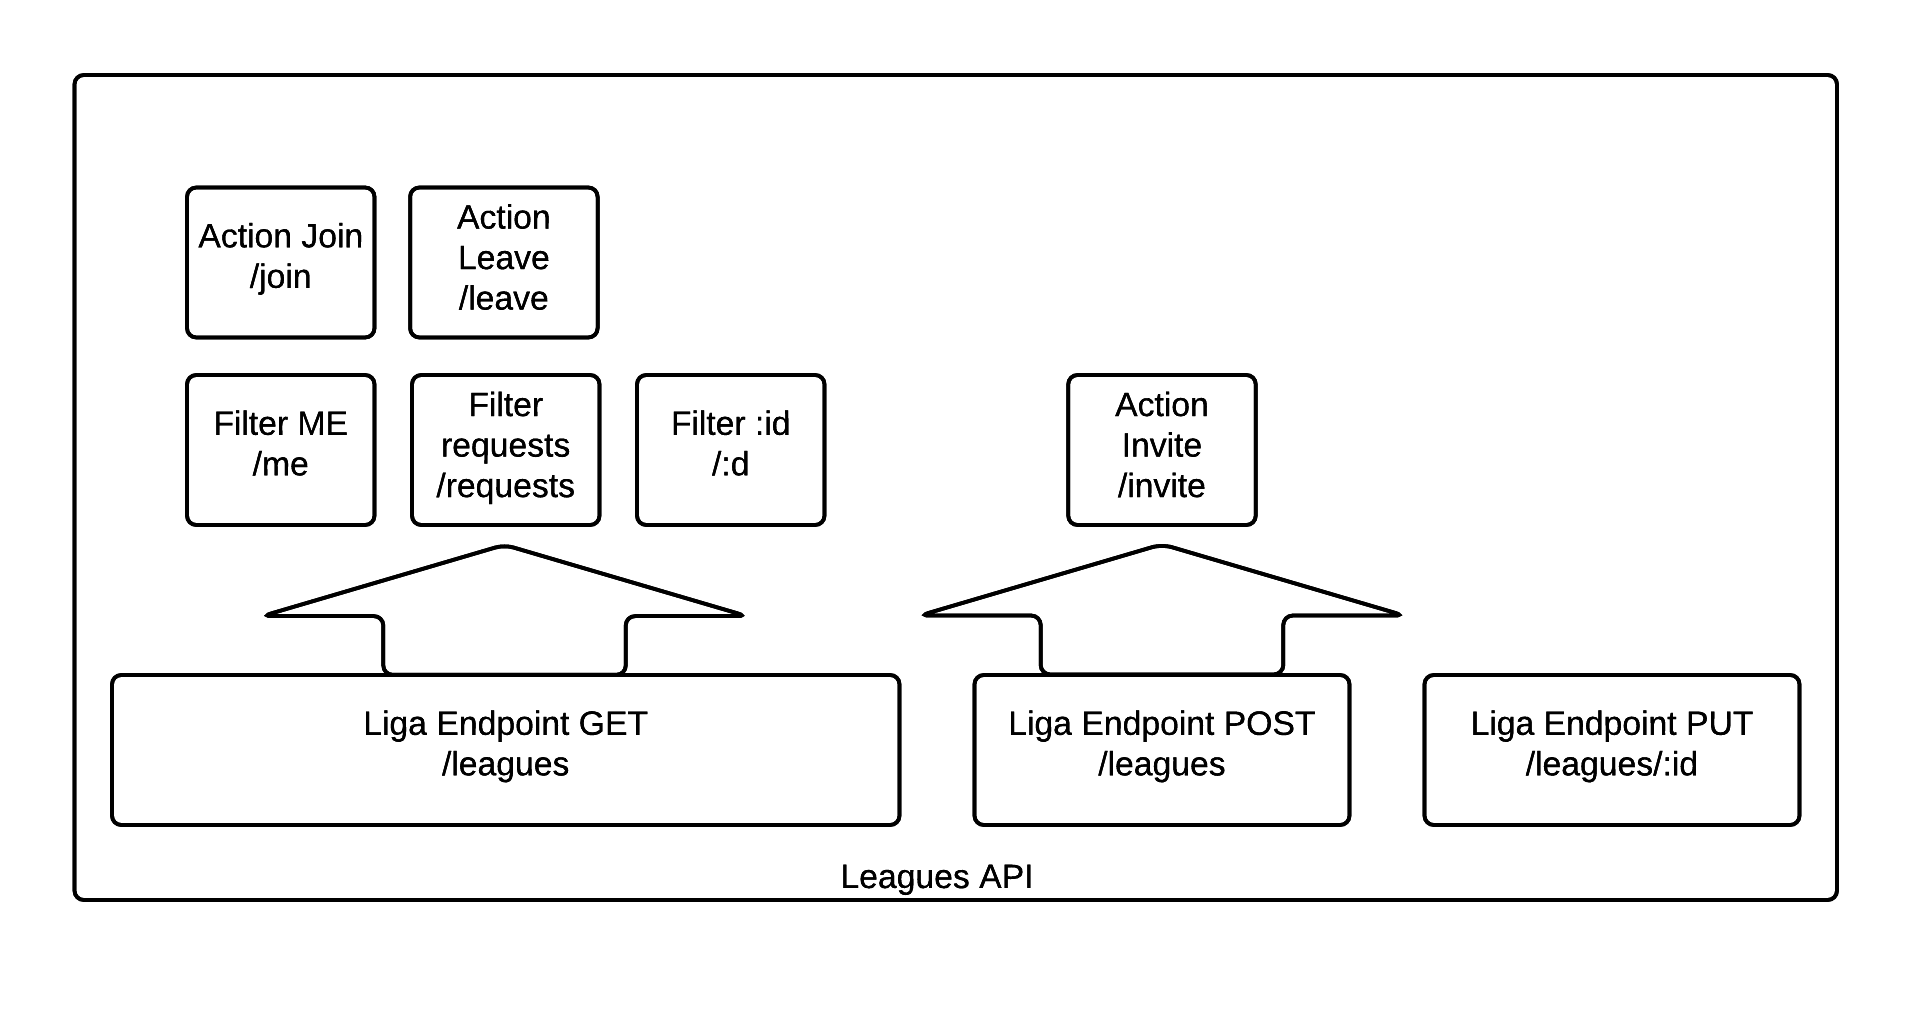
\includegraphics[width=0.8\textwidth]{Graphics/api_league.png}
	\caption{API f�r Ligen}
	\label{LeagueAPI}
	\end{figure}

Bei der Liga gibt es - wie bei allen Endpunkten - CRUD Endpunkte (/leagues f�r list all, /leagues/:id f�r Show Element, POST /leagues f�r Create League, PUT /leagues/:id f�r Update League). Zus�tzlich gbit es eine Join Action, welche den authentisierten User einer Liga hinzuf�gt sowie ein Leave Endpunkt um die Registriertung zu l�schen.

Ein zus�tzlicher Endpunkt ist /leagues/invite, welcher erm�glicht einen User zu einer Liga einzuladen.

\subsubsection{Codebeispiel - Join/Leave Funktionen}

Die Join/Leave Funktionalit�t besteht aus zwei API Endpunkten. Wenn man nun die URL /leagues/join aufruft, wird folgender Code ausgef�hrt:

\begin{lstlisting}
exports.join = function (req, res) {

    var league = req.league;
    var user = req.user;
    var userToPoints = new UserToPoints();
    userToPoints.user = req.user;
    userToPoints.save();

    league.users.push(userToPoints);
    user.leagues.push(league)

    console.log(league);
    league.save(function (err) {
        ....
\end{lstlisting}

Auf der Zeile 3 und 4 werden User und Liga aus dem Request gelesen. Diese Daten werden implizit von AngularJS mitgeliefert. 

Nun wird ein neues Liga-Spieler Objekt, ein Objekt welches den Spieler und seine Ranglistenpunkte beinhaltet erstellt und gespeichert (Zeile 5-7). Dieses Objekt wird nun in die Liste aller Liga-Spieler Objekte hinzugef�gt und die Liga wird abgespeichert (Zeile 13).

\begin{lstlisting}
exports.leave = function (req, res) {
    var league = req.league;
    var user = req.user;
    var i = league.users.indexOf(req.user);
    league.users.splice(i, 1);
    var j = user.leagues.indexOf(req.league);
    user.leagues.splice(j, 1);
    league.save(function (err) {
    ....
\end{lstlisting}
Will ein User die Liga verlassen, wird sein Objekt aus der Liste von Spielern gel�scht.

	\newpage
\subsection{Racketsportzentrum Endpunkt /courts}
\begin{figure}[ht]
	\centering
	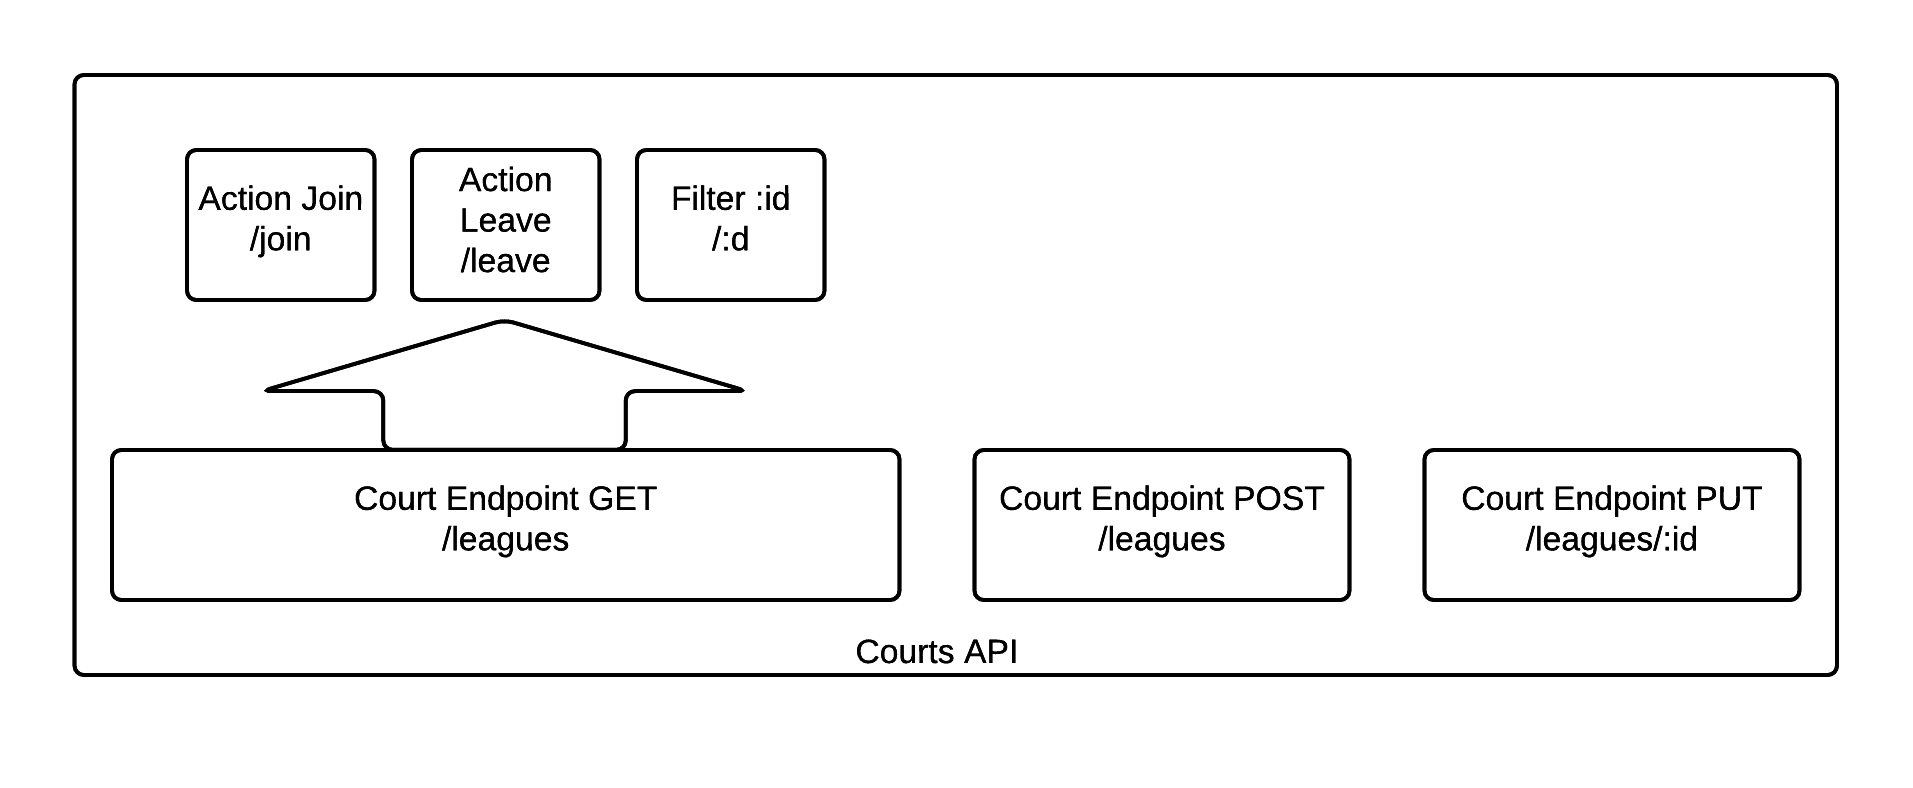
\includegraphics[width=0.8\textwidth]{Graphics/api_court.png}
	\caption{API f�r Racketsportzentren}
	\label{CourtAPI}
\end{figure}
Gleich wie beim Liga Endpunkt gibt es die CRUD Endpunkte sowie ein Join/Leave Endpunkt

\subsection{Benutzer Endpunkt /users}
Neben den �blichen Benutzerverwaltungs Endpunkten (/user/signin, /user/signout, /user signup, /auth/forgot), welche hier nicht Dokumentiert werden, gibt es Endpunkte f�r das Freunde-System:
\begin{itemize}
	\itemsep-0.5em
	\item GET /users/friend - Auflistung aller Freunde
	\item DELETE /users/friend - L�schen eines Freundes
	\item GET /users/request -  Senden eines Freund Requests
	\item DELETE /users/request - L�schen eines Freund Requests
\end{itemize}

\subsubsection{Codebeispiel - OAuth Integration}
Der MEAN Stack bietet ein OAuth Integrations Plugin an. Man muss nur noch das Plugin konfigurieren. Daf�r wird f�r jeden Authentication Provider eine Strategie definiert:
\begin{lstlisting}
....
	GoogleStrategy = require('passport-google-oauth').OAuth2Strategy,
....
module.exports = function() {
	// Use google strategy
	passport.use(new GoogleStrategy({
			clientID: config.google.clientID,
			clientSecret: config.google.clientSecret,
			callbackURL: config.google.callbackURL,
			passReqToCallback: true
		},
		function(req, accessToken, refreshToken, profile, done) {
			// Set the provider data and include tokens
			var providerData = profile._json;
			providerData.accessToken = accessToken;
			providerData.refreshToken = refreshToken;

			// Create the user OAuth profile
			var providerUserProfile = {
				firstName: profile.name.givenName,
				lastName: profile.name.familyName,
				displayName: profile.displayName,
				email: profile.emails[0].value,
				username: profile.username,
				provider: 'google',
				providerIdentifierField: 'id',
				providerData: providerData
			};

			// Save the user OAuth profile
			users.saveOAuthUserProfile(req, providerUserProfile, done);
		}
	));
};
\end{lstlisting}

Die Daten werden bei Registrierung �ber OAuth in das Userprofil abgelegt. (Siehe Zeile 19-27 ). Zus�tzlich ist es n�tig bei jedem Provider ein Access Token anzufordern und in die Produktionsumgebung der Applikation einzupflegen.

\section{Web Applikation}

Die WebApplikation ist wie bereits erw�hnt mit Bootstrap und AngularJS programmiert. In AngularJS werden Direktiven erstellt, um einzelne API Endpunkte anzusprechen und diese Realtime in die View zu injecten. Hier ein Beispiel einer Direktive:
\begin{lstlisting}
$scope.find = function() {
			$scope.courts = Courts.query();
		};

\end{lstlisting}

Wenn die Operation find() in der View aufgerufen wird, erstellt AngularJS eine Query zum Endpunkt /courts und bekommt alle Court Objekte zur�ck. Diese Courtobjekte werden nun in die globale Variable courts im \textdollar scope abgef�llt. AngularJS updatet nun die View, welche die Variable courts anzeigt:
\begin{lstlisting}
<section data-ng-controller="CourtsController" data-ng-init="find()">
    ....
        <table id="courtslist" class="table">
            <tr>
                <th>Name</th><th>Adresse</th><th>Verf�gbare Sportarten</th>
            </tr>

            <tr data-ng-repeat="court in courts" id="{{court._id}}" ng-click="go(court)"  onMouseover="this.bgColor='#DDDDDD'" onMouseout="this.bgColor='#FFFFFF'">
                <td data-ng-bind="court.name"></td>
                <td data-ng-bind="court.address"></td>
                <td data-ng-bind="court.sports"></td>
            </tr>
        </table>
....
\end{lstlisting}

Das ganze Webinterface ist auf solchen Direktiven aufgebaut.

\subsection{Google Maps Integration}
 Eine Adresse wie z.B. \lq Vitis \rq hat das Problem, dass man geographische N�he suchen kann. Darum ist es wichtig, das die Racketsport zentren ein Geographisch Valides Objekt haben. Um dies zu erreichen wurde die API von Google Maps integriert. Der Benutzer muss nun noch einem Objekt in Google Maps suchen, und dieses Selektieren um eine Valide Addresse zu bekommen. Folgendes Formularelement existiert in der View:
 \begin{lstlisting}
 <div class="form-group">
   <label for="address">Adresse</label>
   <input type="text" onFocus="geolocate()" id="address" name="address" class="form-control" data-ng-model="address" required>
 </div>
 \end{lstlisting}
 
 Wie auf Zeile 3 ersichtlich wird die direktive geolocate() aufgerufen. Diese Funktion ist Bestandteil der Google API, welche im Header von \url{https://maps.googleapis.com/maps/api/js?v=3.exp&signed_in=true&libraries=places} gedownloadet wird. Die ID address wird von dem Court Controller aufgerufen und folgender Listener wird hinzugef�gt:
 \begin{lstlisting}
 var placeSearch, autocomplete;
 		if(document.getElementById('address')) {
 			autocomplete = new google.maps.places.Autocomplete(
 				/** @type {HTMLInputElement} */(document.getElementById('address')));
 			// When the user selects an address from the dropdown,
 			// populate the address fields in the form.
 
 			google.maps.event.addListener(autocomplete, 'place_changed', function () {
 				$scope.updateAddress();
 			});
 		}
 \end{lstlisting}
Der autocomplete Listener ruft nun die AngularJS direktive updateAddress() auf:

\begin{lstlisting}
$scope.updateAddress =function() {
			var place = autocomplete.getPlace();
			document.getElementById('address').value = place.formatted_address;
			document.getElementById('lat').value = place.geometry.location.A;
			document.getElementById('lng').value = place.geometry.location.F;
			if ($scope.court) {
				$scope.court.address = place.formatted_address;
				$scope.court.lat = place.geometry.location.A;
				$scope.court.lng = place.geometry.location.F;
			}else{
				this.address = place.formatted_address;
				this.lat = place.geometry.location.A;
				this.lng = place.geometry.location.F;
			}
		};
\end{lstlisting}

UpdateAddress sucht das Google Maps Objekt und speichert die Values - Addresse sowie Koordinaten - in die View. Bei dem Abschicken des Formulares wird nun gepr�ft ob die Koordinaten existieren, falls nicht, ist es keine valide Adresse, wie man im Court-Model sieht (Zeile 3 und 7):
\begin{lstlisting}
lat: {
		type: String,
		required: "Please fill in a correct address (select it from the dropdown)"
	},
lng: {
		type: String,
		required: "Please fill in a correct address (select it from the dropdown)"
	}
\end{lstlisting}


\section{Android Applikation}
Als Grundlage f�r die Android Applikation wurde eine Applikation von gonative.io generiert. Im Laufe des Projektes - nach erheblicher �berschreitung des vorgeschriebenen Aufwandes - wurde entschieden keine vollst�ndig Native Webapplikation zu erstellen. Stattdessen wird eine WebView erstellt, welche die Mobile Webseite darstellt. Um alle Funktionalit�t zu behalten, wird �ber die WebView und Interception Algorithmen Push-Nachriten erm�glicht. Der einzige Setback ist, das die Website offline nicht verf�gbar ist.

\subsubsection{Codebeispiel - Push Interception}
TBD!!!!


\section{Workflows}
\section{Allgemeine Workflows}
\subsection{CRUD f�r Datenobjekte}
Alle Datenobjekte haben einen Endpunkt. Jeder Endpunkt stellt CRUD Operationen zur Verf�gung:
\begin{itemize}
	\itemsep -0.5em
	\item C - Neues Objekt erstellen
	\item R - Ein Objekt anzeigen
	\item U - Ein Objekt aktualisieren
	\item D - Ein Objekt l�schen
	\end{itemize}
	
	Zus�tzlich wird noch einen Endpunkt zur Auflistung aller Objekte angeboten. 

\newpage
\section{Court}
\subsection{Court Registrierung}
Wenn der User den Knopf im User Interface zur Registrierung das Racketsportzentrums dr�ckt, wird im Hintergrund der /courts/join API Call ausgef�hrt. Dieser Call f�gt der User der Anfrage in ein Array - bestehend aus allen registrierten Usern - ein. 
\begin{figure}[ht]
	\centering
	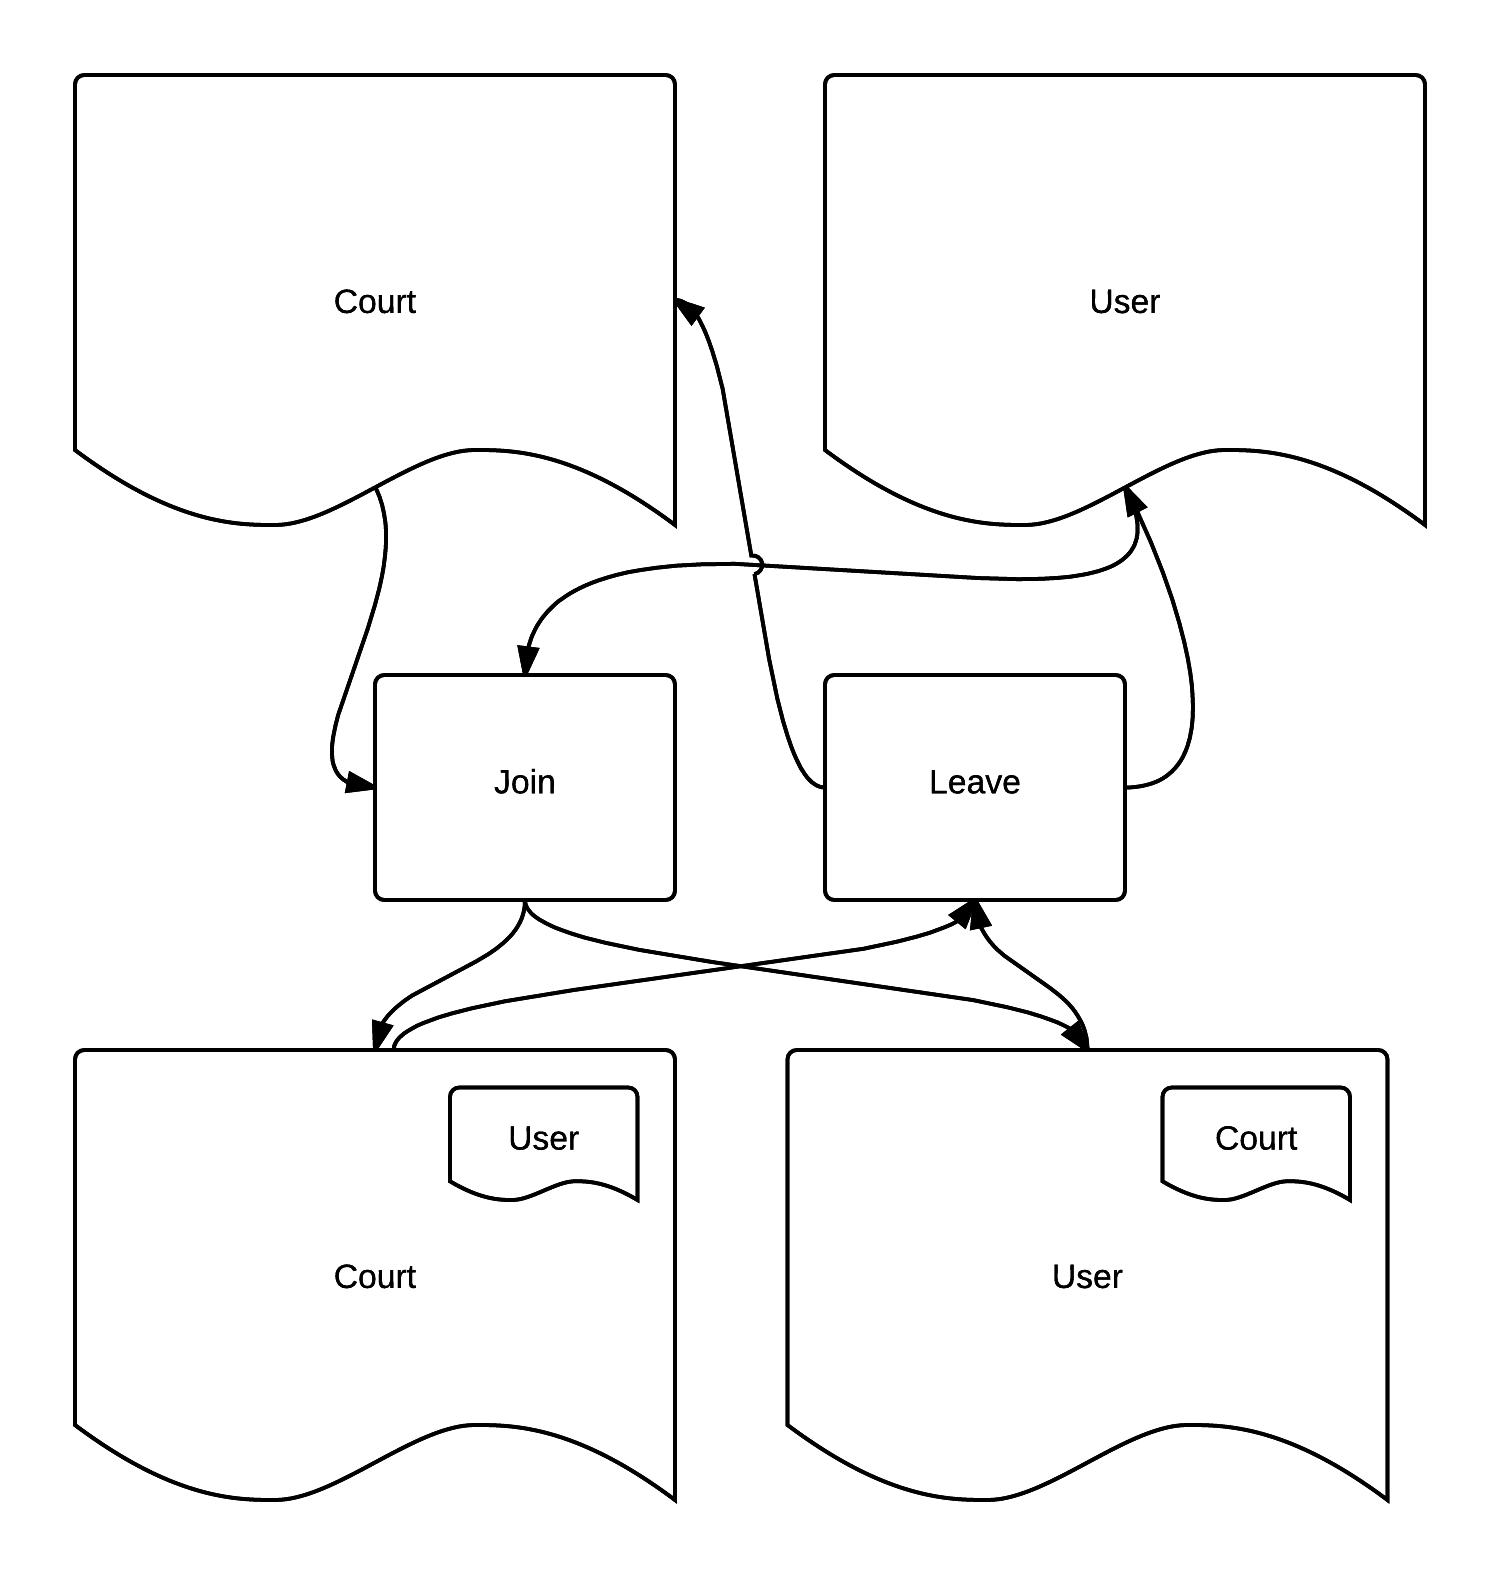
\includegraphics[width=0.7\textwidth]{Graphics/workflow_court.png}
	\caption{Racketsportzentrum Workflow}
	\label{CourtWorkflow}
\end{figure}
\newpage

\section{Liga}
\subsection{Liga Registrierung}
Identisch zu der Court Registrierung funktioniert die Liga Registrierung
\begin{figure}[ht]
	\centering
	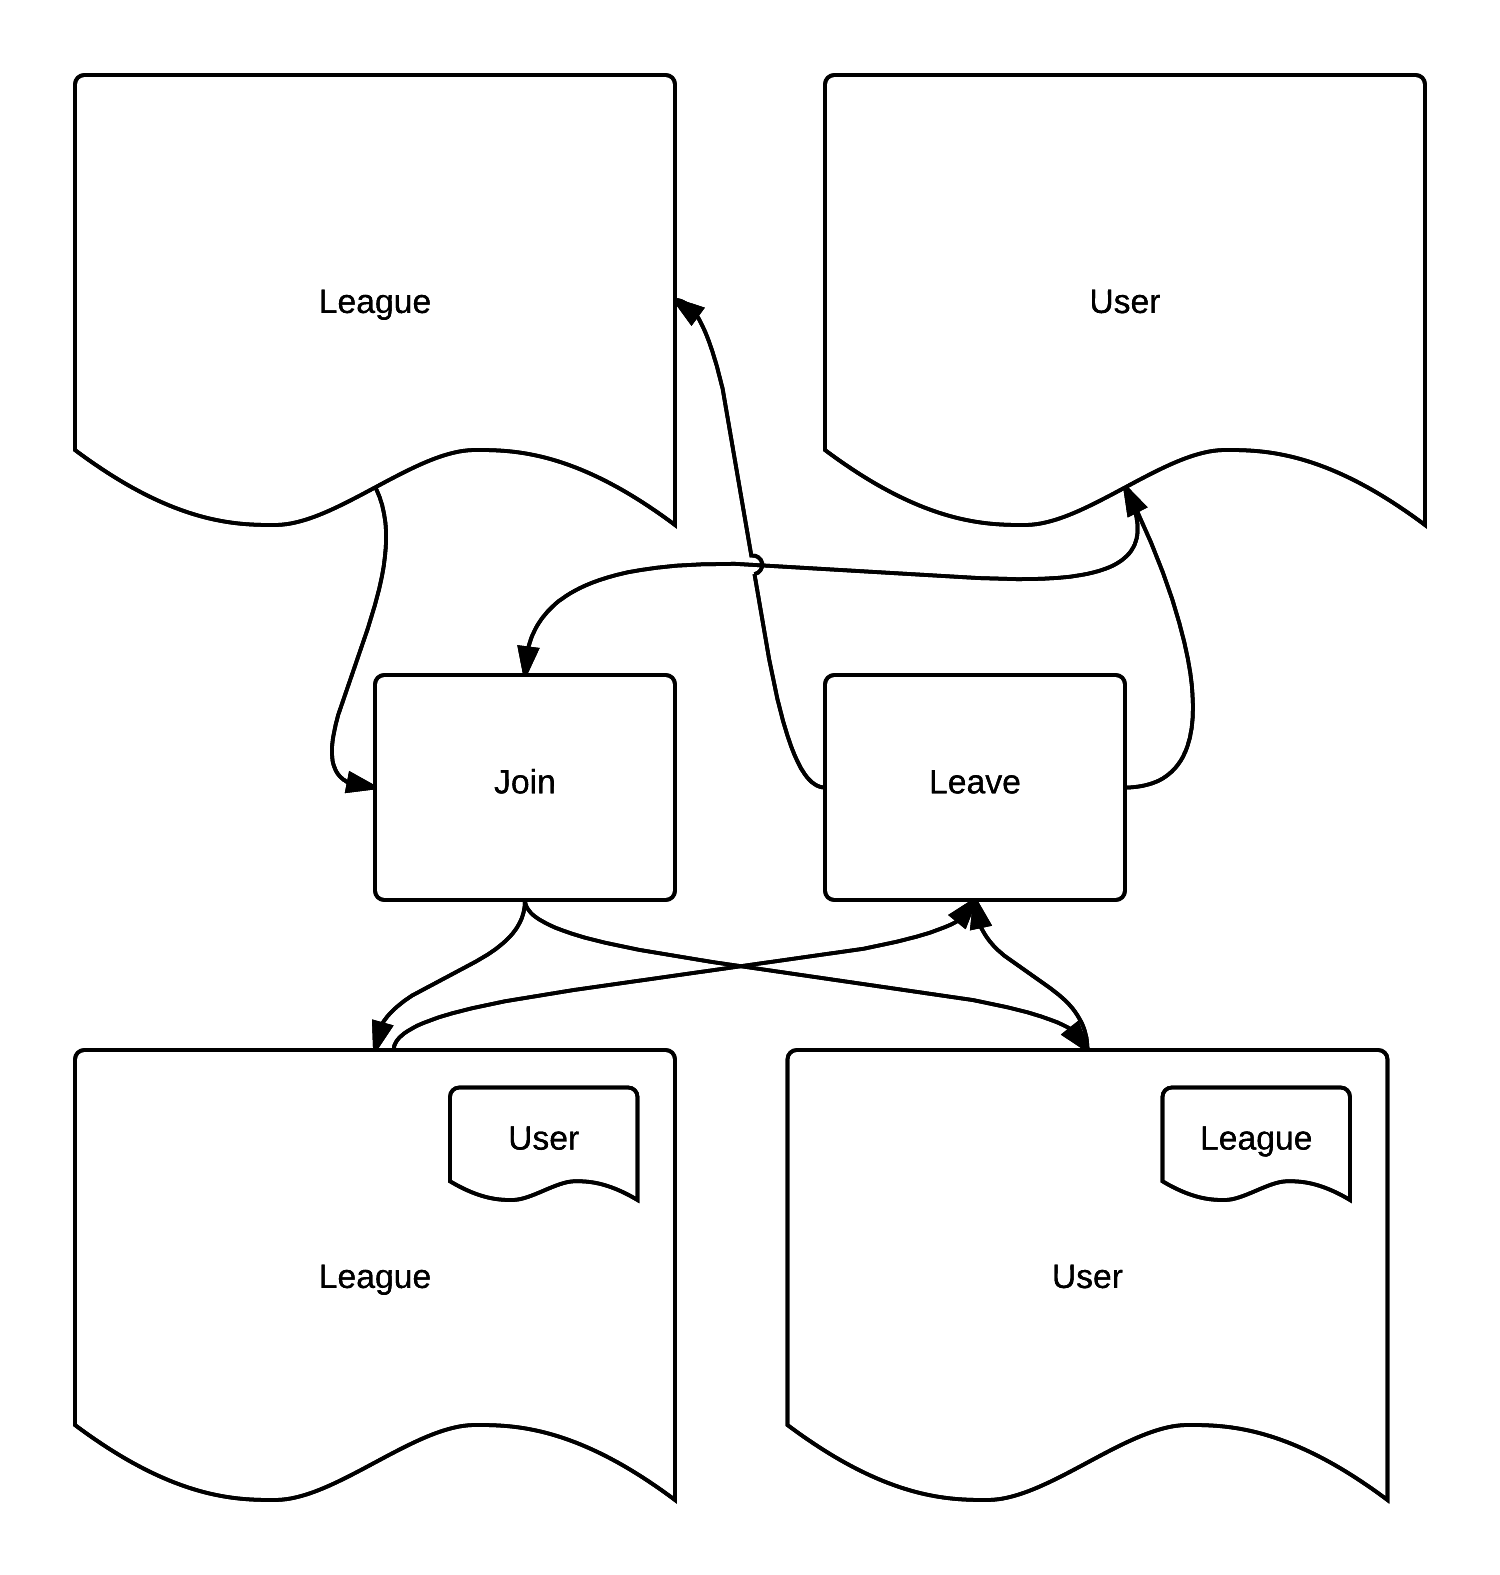
\includegraphics[width=0.7\textwidth]{Graphics/workflow_league.png}
	\caption{Liga Workflow}
	\label{LegueWorkflow}
\end{figure}

	\newpage
	\subsection{Automatische Herausforderung Liga}
	
	Bei der erstellung einer Liga kann ausgew�hlt werden ob automatische Herausforderungen aktiviert werden sollten. Aktuell gibt es vier verschiedene ausw�hlbare Modi:
	\begin{itemize}
		\item Weeklyall: W�chentliche Herausforderung, jeder gegen jeder, zuf�lliger Gegner
		\item Biweeklyall: Herausforderung alle zwei Wochen, jeder gegen  jeder, zuf�lliger Gegner
		\item WeeklyTopTwo: Herausforderung jede Woche, immer die zwei N�chsten in der Rangliste
		\item BiweeklTopTwo: Herausforderung alle zwei Wochen, immer die zwei N�chsten in der Rangliste
	\end{itemize}
	\begin{figure}[ht]
		\centering
		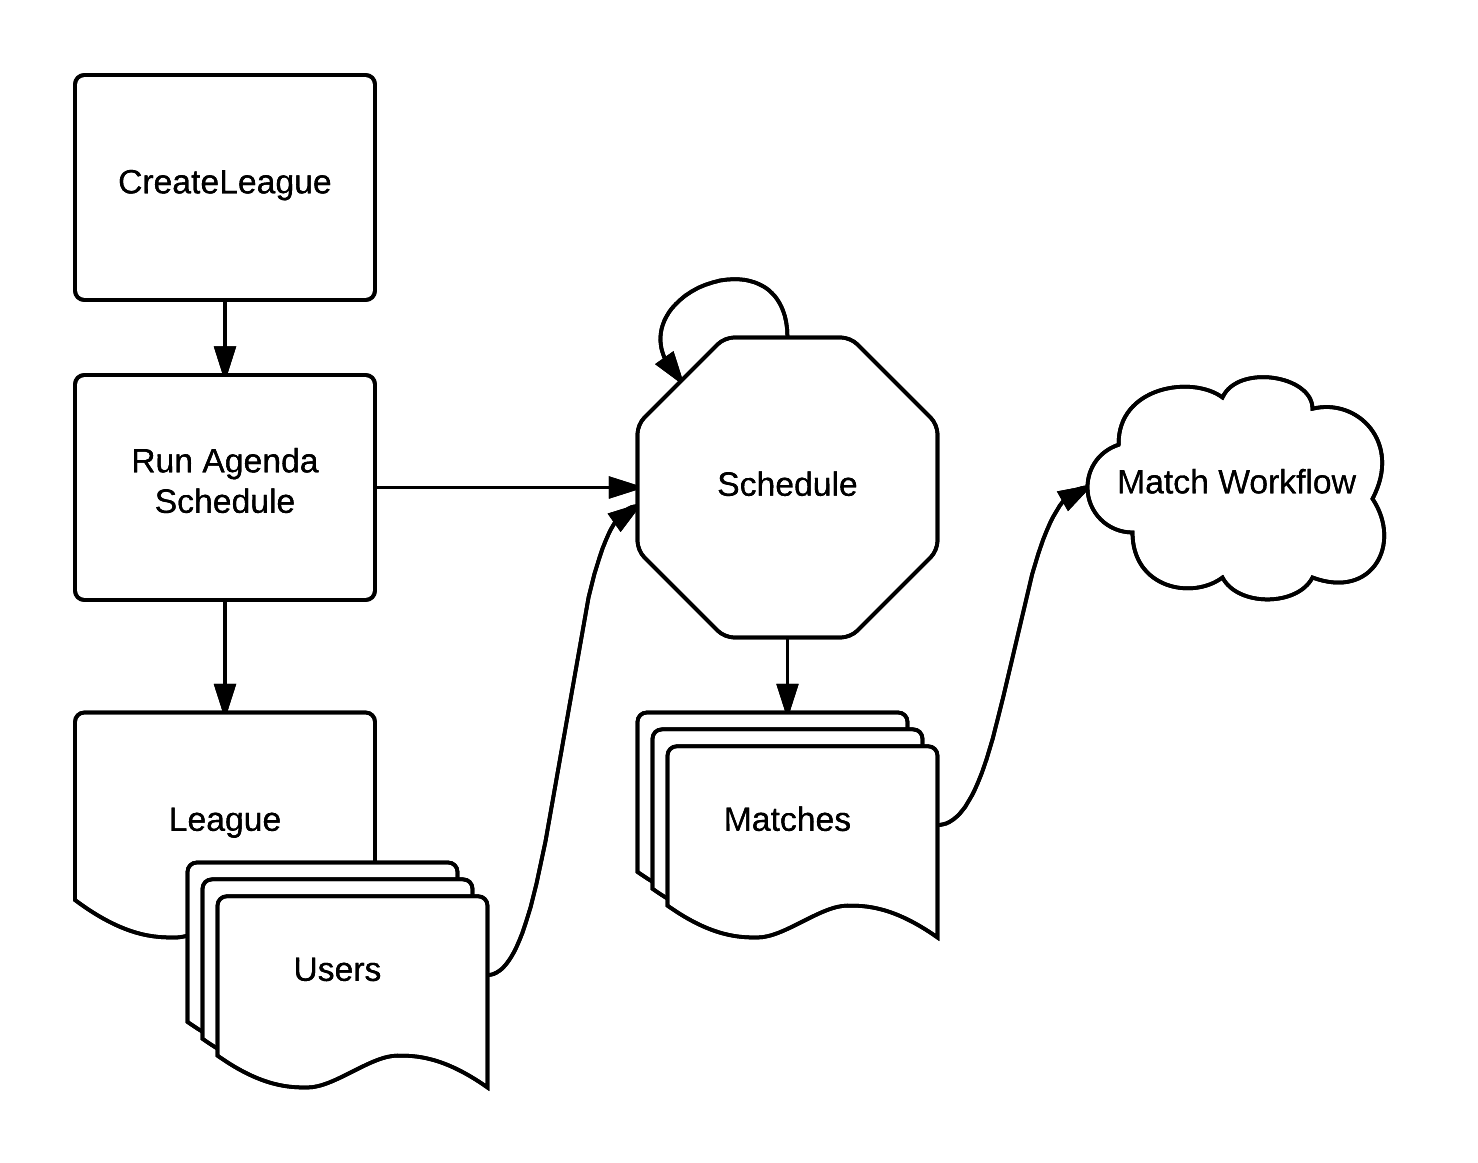
\includegraphics[width=0.7\textwidth]{Graphics/schedue_workflow.png}
		\caption{Schedule Workflow}
		\label{ScheduleWorkflow}
	\end{figure}
	\newpage
	\subsubsection{Codebeispiel - Scheduling}
	F�r das  Scheduling wird eine Externe Scheduling Libary f�r NodeJS gebraucht. Diese Library wird in den Startup der Applikation eingebunden:
\begin{lstlisting}
	var agenda = new Agenda({db: {address: config.dbagenda}});
	console.log("starting agenda");
	app.use('/agenda-ui', agendaUI(agenda, {poll: 1000}));
	agenda.start();
\end{lstlisting}
	Die Scheduling Libary - weiterf�hren Referenziert mit dem Namen Agenda - ben�tzt nun MongoDB um die Schedules zu persistieren. Wenn nun eine Liga erstellt wird, wird angegeben ob man Automatische Herausforderungen w�nscht. Falls dies gew�nscht ist, wird in der Funktion bei der Erstellung der Liga das Scheduling eingerichtet:
	\begin{lstlisting}
	if(league.requestShedule){
	    var agenda = new Agenda({db: {address: config.dbagenda}})
	    console.log("execute schedulematches sending ID: "+ league);
	    agenda.define(league._id+' schedule', League.scheduleMatches);
	    var job = agenda.create(league._id+' schedule',league.id);
	    if(league.requestShedule == 'weeklyAll'){
	        job.repeatAt('in 1 weeks');
	    }
	    if(league.requestShedule == 'biweeklyAll'){
	        job.repeatAt('in 2 weeks');
	    }
	    if(league.requestShedule == 'biweeklyTwoTop'){
	        job.repeatAt('in 2 weeks');
	    }
	    if(league.requestShedule == 'weeklyTwoTop'){
	        job.repeatAt('in 1 weeks');
	    }
	
	    //agenda.every('10 minutes', league._id+' schedule', league.id);
	
	    job.save()
	    agenda.start();
	}
	\end{lstlisting}
	
	\subsubsection{Random Herausforderungen / Rang Herausforderungen}
	Das Scheduling hat nun keinen Kontext der Applikation. Es beinhaltet nur das Model sowie alle Funktionen des Models. Aus diesem Grund wurde eine Funktion f�r das Starten der Herausforderungen innerhalb des Models erstellt:
	\begin{lstlisting}
	LeagueSchema.statics.scheduleMatches = function(job){
	    var League = mongoose.model('League'),
	        UserToPoints = mongoose.model('UserToPoints'),
	        Matches = mongoose.model('Match');
	    var leagueid = job.attrs.data;
	    League.findById(leagueid).populate("users").exec(function(err, league) {
	        UserToPoints.populate(league.users, {path: 'user', select: 'username'}, function (err, user) {
	
	            if (league) {
	                var l = league.users.length;
	                var player1, player2;
	                var k = league.users.length;
	                while (true){
	                if(league.requestShedule == 'biweeklyTwoTop' || league.requestShedule == 'weeklyTwoTop' ) {
	
	                        if (league.users.length > 1) {
	                             player1 = league.users[0].user;
	                            player2 = league.users[1].user;
	                            leage.users.splice(0,2);
	                        }
	                        else {
	                            break;
	                        }
	
	                }else {
	
	                        if (league.users.length > 1) {
	                            var p1 = Math.floor(Math.random() * l);
	                             player1 = league.users[p1].user;
	                            league.users.splice(p1, 1);
	                            l--;
	                            var p2 = Math.floor(Math.random() * l);
	                             player2 = league.users[p2].user;
	                            league.users.splice(p2, 1);
	                            l--;
	
	                        }
	                        else {
	                            break;
	                        }
	
	                    }
	                    var match = new Matches();
	                    match.spieler.push({user: player1});
	                    match.spieler.push({user: player2});
	                    match.sport = league.sport;
	                    match.league = league;
	                    match.state = 'new';
	                    match.save(function (err) {
	                        if (err) {
	                            console.log(err);
	                        }
	                    });
	                    if (l == 0) {
	                        break;
	                    }
	                }
	
	            } else {
	                console.log("no league with ID " + leagid + " found");
	            }
	        });
	    }
	    );
	
	}
	\end{lstlisting}
	Bis zur Zeile 9 sucht sich nun diese statische Funktion der Kontext aus der Datenbank zusammen. Es sucht sich selber, popularisiert die User und startet ab Zeile 14 das erstellen von Herausforderungen. 
	
	Je nach Modus (Random Herausforderungen, oder nach Rangliste) wird nun der Rangliste nach Spieler herausgefordert und diese aus der Rangliste gel�scht. Da das Liga Objekt nicht gespeichert wird, sind die �nderungen der Rangliste nur tempor�r. 
	
	Ist nun der Modus Random, wird das ganze etwas Komplexer. Zuerst wird aus der Rangliste ein Spieler zuf�llig ausgew�hlt (Zeile 28). Dieser Spieler wird nun von der Liste gel�scht und der Zeite Spieler wird ausgew�hlt (Zeile 32). Dieser wird nun auch gel�scht und der Match zwischen den zwei Spielern wird vereinbart. Das ganze wiederholt sich, bis keine Spieler mehr in der Rangliste sind. 
	
\begin{landscape}

\section{Match}
\subsection{Match Workflow}
Der Matchworkflow ist das Hauptelement der Applikation. Der Workflow regelt, wie der Match als Business Prozess durchgef�hrt wird. 
\begin{figure}[ht]
	\centering
	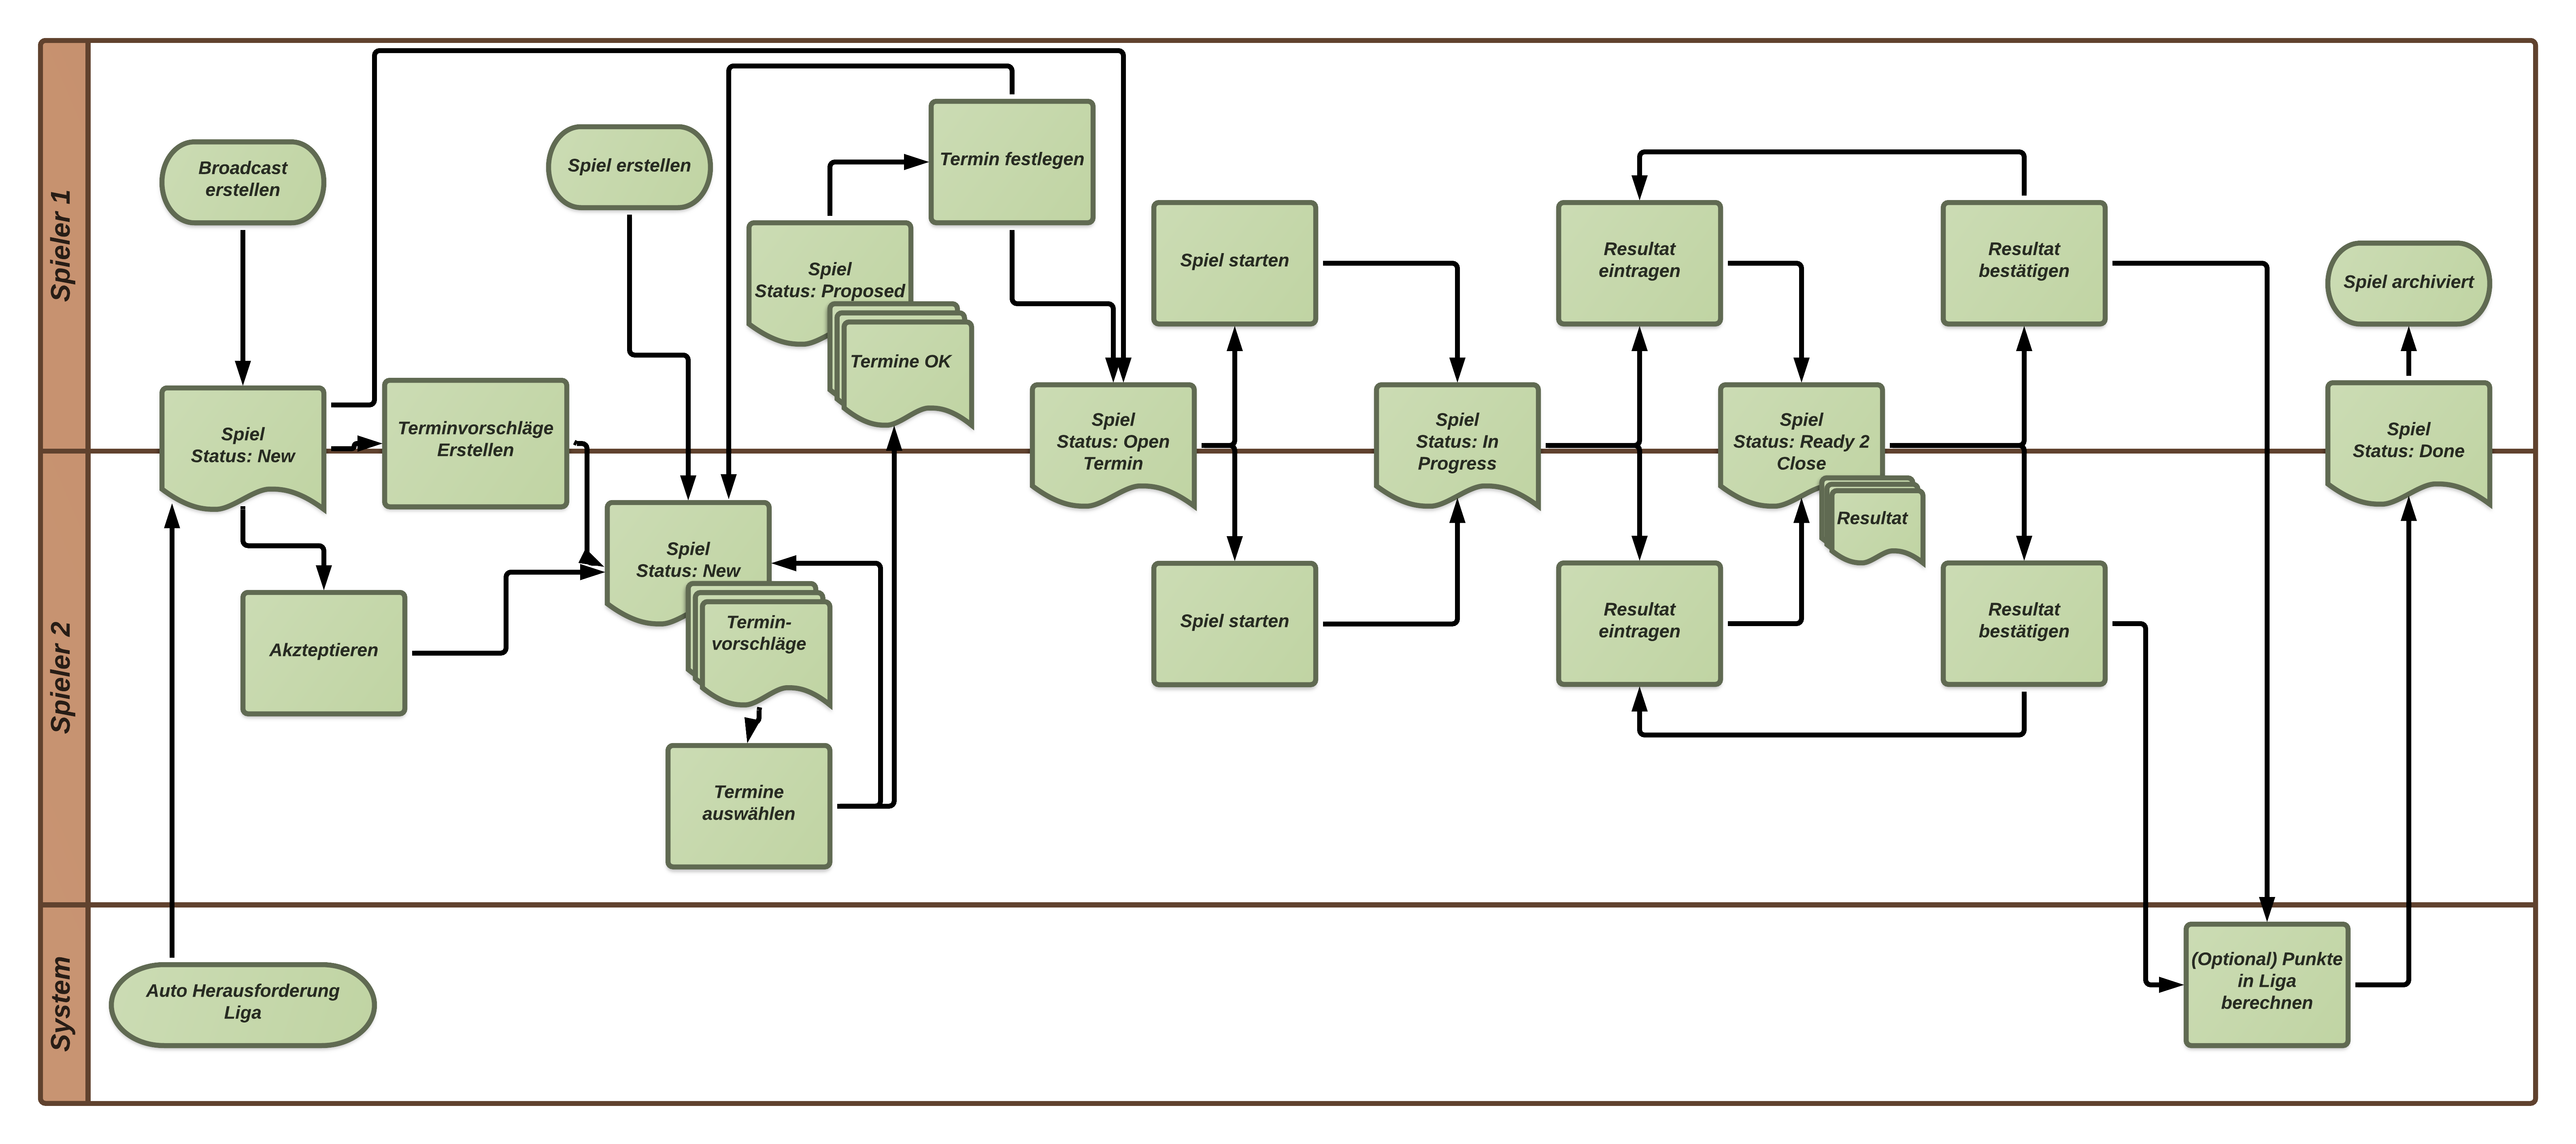
\includegraphics[width=1.3\textwidth]{Graphics/match_workflow.png}
	\caption{Spiel Workflow}
	\label{MatchWorkflow}
\end{figure}
\end{landscape}

Der Workflow wird �ber drei verschiedene F�lle gestartet: 
\begin{itemize}
	\itemsep -0.5em
	\item Das System erstellt Auto-Herausforderungen f�r die Liga
	\item Der User erstellt ein Broadcast Spiel
	\item Der User erstellt ein regul�res spiel.
	
	\end{itemize}
	
Wenn der User ein \textbf{regul�res Spiel} erstellt, sind beide Spieler, sowie Terminvorschl�ge schon definiert. Es folgt die Aktion \grqq Termin ausw�hlen\grqq.

Erstellt der User ein \textbf{broadcast Spiel}, hat das Spiel den Status \grqq New\grqq, jedoch noch keinen zweiten Spieler definiert. Zus�tzlich werden keine Terminvorschl�ge ausgef�llt, sondern einen fixen Termin. Akzeptiert jemand den Broadcast wird der zweite Spieler eingetragen und der Status �ndert sich direkt auf Open.
 
Sind User in einer Liga, erstellt die \textbf{Liga eine Herausforderung}. Das Spiel enth�lt kein Court und keine Terminvorschl�ge. Der User muss nun Terminvorschl�ge ausf�llen und ein Court definieren. 

Anschliessend haben alle Use Cases den gleichen Workflow. Ist das Spiel und der Termin definiert. Geht der Status des Spiels zu \grqq Open\grqq . Danach kann von beiden Spielern der Status auf \grqq In progress\grqq gesetzt werden. Beide k�nnen ein Resultat eintragen. Der jeweil andere Spieler best�tigt anschliessend das Resultat. Bei der Best�tigung des Resultats wird das Spiel archiviert und optional die Rangliste der Liga aktualisiert.
\newpage

\section{User}
\subsection{Freunde System}
\begin{figure}[ht]
	\centering
	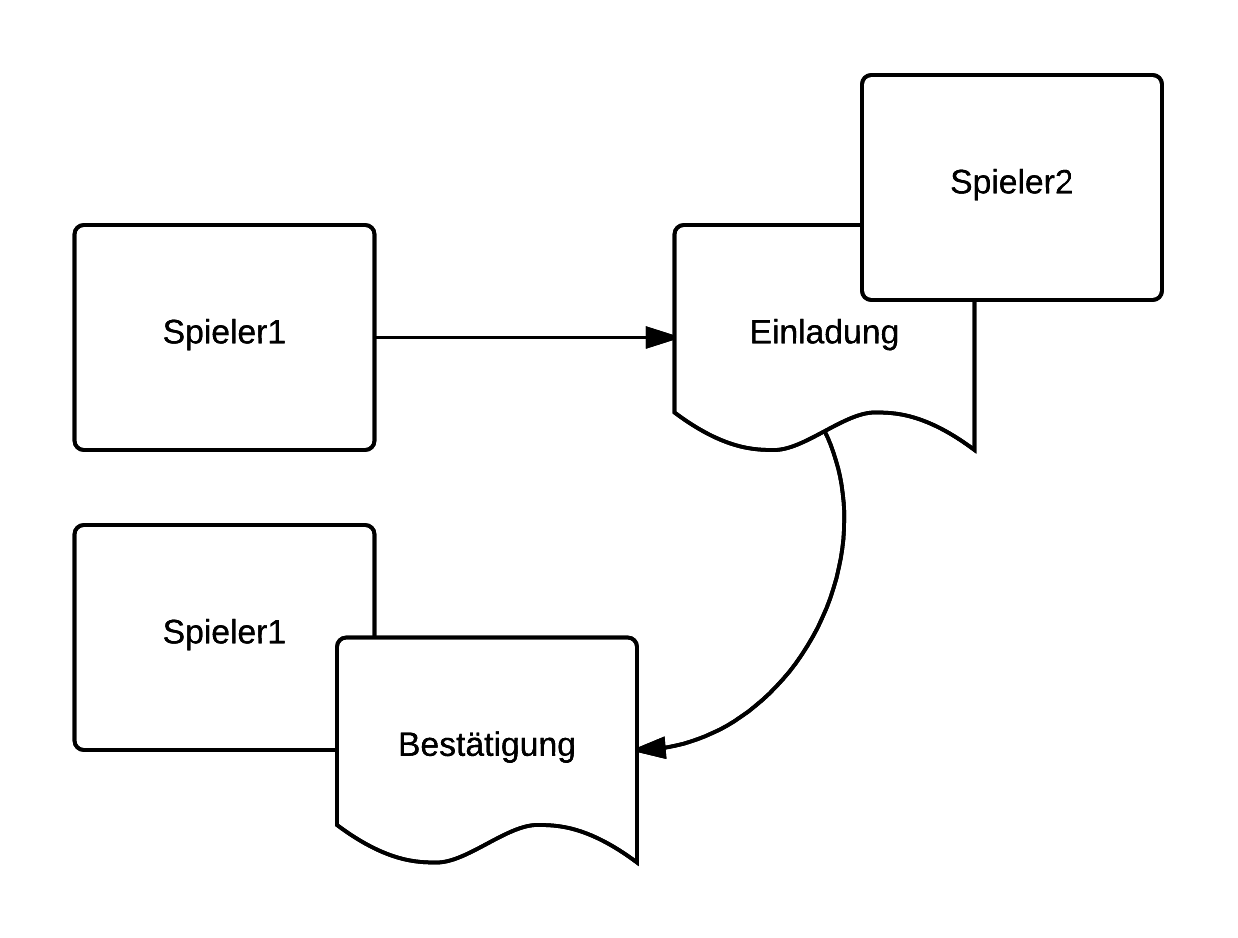
\includegraphics[width=0.7\textwidth]{Graphics/friendworkflow.png}
	\caption{Freunde Workflow}
	\label{FriendWorkflow}
\end{figure}
\FloatBarrier
Spieler1 sendet eine Einladung zur Freundschaft an Spieler 2. Diese Einladung ist eine Liste bei Spieler2 sowie bei Spieler1:
\begin{lstlisting}
friendrequests: [{
		type: Schema.ObjectId,
		ref: "User"
	}],
\end{lstlisting}
Bei der Best�tigung der Einladung tr�gt sich Spieler2 sowie Spieler1 das User-Objekt von dem friendrequests Feld in das friends Feld:
\begin{lstlisting}
friends: [{
		type: Schema.ObjectId,
		ref: "User"
	}],
\end{lstlisting}
\end{normalsize}

\listoffigures

\printbibliography
\end{spacing}
\end{document}
